	
\documentclass[svgnames]{beamer}

\mode<presentation> {
\usetheme{Warsaw}
}

\usepackage{graphicx}
\usepackage{booktabs}
\usepackage{listings}
\usepackage{color}
%\usepackage[lofdepth,lotdepth]{subfig}
\usepackage{subfig}
\usepackage{fontawesome}
\usepackage{hyperref}

\definecolor{codegreen}{rgb}{0,0.6,0}
\definecolor{codegray}{rgb}{0.5,0.5,0.5}
\definecolor{codepurple}{rgb}{0.58,0,0.82}
\definecolor{backcolour}{rgb}{0.95,0.95,0.92}

\beamertemplatenavigationsymbolsempty


\lstdefinestyle{mystyle}{
    backgroundcolor=\color{backcolour},   
    commentstyle=\color{codegreen},
    keywordstyle=\color{magenta},
    numberstyle=\tiny\color{codegray},
    stringstyle=\color{codepurple},
    %basicstyle=\footnotesize,
    basicstyle=\scriptsize\ttfamily,
    breakatwhitespace=false,         
    breaklines=true,                 
    captionpos=b,                    
    keepspaces=true,                 
    numbers=left,                    
    numbersep=5pt,                  
    showspaces=false,                
    showstringspaces=false,
    showtabs=false,                  
    tabsize=2,
    language=bash
}

\definecolor{RRR}{rgb}{0.702,0.2,0.2}
\definecolor{bleuclair}{rgb}{0.9,0.9,1}
\definecolor{grisbleu}{rgb}{0.85,0.85,1}
\definecolor{monbleu}{rgb}{0,0.4,0.6}
\definecolor{bleuclair}{rgb}{0.9,0.9,1}
\definecolor{autrebleu}{rgb}{0.15,0.5,0.65}
\definecolor{bleufond}{rgb}{0.59,0.66,0.81}
\definecolor{bleufondplus}{rgb}{0.21,0.29,0.47}
\definecolor{monrouge}{rgb}{1,0.16,0.14}
\definecolor{denim}{rgb}{0.08, 0.38, 0.74}
 \definecolor{cornflowerblue}{rgb}{0.39, 0.58, 0.93}

\definecolor{flame}{rgb}{0.89, 0.35, 0.13}
\hypersetup{colorlinks,linkcolor=,urlcolor=cornflowerblue}
\newcommand{\code}[1]{\textit{\ttfamily\textcolor{flame}{#1}}}


%\setbeamercolor{normal text}{bg=white}
%\setbeamercolor{alerted text}{fg=red}
% \setbeamercolor{example text}{fg=green!50!black}
% \setbeamercolor{structure}{fg=beamer@blendedblue}
\setbeamercolor{background canvas}{bg=white}
% \setbeamercolor{background}{bg=green, fg=red}
% \setbeamercolor{palette primary}{use=structure,fg=structure.fg}
% \setbeamercolor{palette secondary}{use=structure,fg=structure.fg!75!black}
% \setbeamercolor{palette tertiary}{use=structure,fg=structure.fg!50!black}
% \setbeamercolor{palette quaternary}{fg=black}
% \setbeamercolor{palette sidebar primary}{use=normal text,fg=normal text.fg}
% \setbeamercolor{palette sidebar secondary}{use=structure,fg=structure.fg}
% \setbeamercolor{palette sidebar tertiary}{use=normal text,fg=normal text.fg}
% \setbeamercolor{palette sidebar quaternary}{use=structure,fg=structure.fg}
% \setbeamercolor{math text}{}
% \setbeamercolor{math text inlined}{parent=math text}
% \setbeamercolor{math text displayed}{parent=math text}
% \setbeamercolor{normal text in math text}{}
% \setbeamercolor{local structure}{parent=structure}
% \setbeamercolor{titlelike}{parent=structure}
% \setbeamercolor{title}{parent=titlelike}
% \setbeamercolor{title in head/foot}{parent=palette quaternary}
% \setbeamercolor{title in sidebar}{parent=palette sidebar quaternary}
% \setbeamercolor{subtitle}{parent=title}
% \setbeamercolor{author}{}
% \setbeamercolor{author in head/foot}{parent=palette primary}
% \setbeamercolor{author in sidebar}{use=palette sidebar tertiary,fg=palette sidebar tertiary.fg}
% \setbeamercolor{institute}{}
% \setbeamercolor{institute in head/foot}{parent=palette tertiary}
% \setbeamercolor{institute in sidebar}{use=palette sidebar tertiary,fg=palette sidebar tertiary.fg}
% \setbeamercolor{date}{}
% \setbeamercolor{date in head/foot}{parent=palette secondary}
% \setbeamercolor{date in sidebar}{use=palette sidebar tertiary,fg=palette sidebar tertiary.fg}
% \setbeamercolor{titlegraphic}{}
% \setbeamercolor{part name}{}
% \setbeamercolor{part title}{parent=titlelike}
% \setbeamercolor{section name}{}
% \setbeamercolor{section title}{parent=titlelike}
% \setbeamercolor{section in toc}{parent=structure}
% \setbeamercolor{section in toc shaded}{parent=section in toc}
% \setbeamercolor{section in head/foot}{parent=palette tertiary}
% \setbeamercolor{section in sidebar}{parent=palette sidebar secondary}
% \setbeamercolor{section in sidebar shaded}{use=section in sidebar,fg=section in sidebar.fg!40!bg}
% \setbeamercolor{section number projected}{parent=item projected}
% \setbeamercolor{subsection name}{}
% \setbeamercolor{subsection title}{parent=titlelike}
% \setbeamercolor{subsection in toc}{}
% \setbeamercolor{subsection in toc shaded}{parent=subsection in toc}
% \setbeamercolor{subsection in head/foot}{parent=palette secondary}
% \setbeamercolor{subsection in sidebar}{parent=palette sidebar primary}
% \setbeamercolor{subsection in sidebar shaded}{use=subsection in sidebar,fg=subsection in sidebar.fg!40!bg}
% \setbeamercolor{subsection number projected}{parent={subitem projected}}
% \setbeamercolor{subsubsection in toc}{parent=subsection in toc}
% \setbeamercolor{subsubsection in toc shaded}{parent=subsubsection in toc}
% \setbeamercolor{subsubsection in head/foot}{parent=subsection in head/foot}
% \setbeamercolor{subsubsection in sidebar}{parent=subsection in sidebar}
% \setbeamercolor{subsubsection in sidebar shaded}{parent=subsection in sidebar shaded}
% \setbeamercolor{subsubsection number projected}{parent=subsubitem projected}
% \setbeamercolor{headline}{}
% \setbeamercolor{footline}{}
% \setbeamercolor{sidebar}{}
% \setbeamercolor{sidebar left}{parent=sidebar}
% \setbeamercolor{sidebar right}{parent=sidebar}
% \setbeamercolor{logo}{parent=palette secondary}
% \setbeamercolor{frametitle}{parent=titlelike}
% \setbeamercolor{framesubtitle}{parent=frametitle}
% \setbeamercolor{frametitle right}{parent=frametitle}
% \setbeamercolor{caption}{}
% \setbeamercolor{caption name}{parent=structure}
% \setbeamercolor{button}{use=local structure,bg=local structure.fg!50!bg,fg=white}
% \setbeamercolor{button border}{use=button,fg=button.bg}
% \setbeamercolor{navigation symbols}{use=structure,fg=structure.fg!40!bg}
% \setbeamercolor{navigation symbols dimmed}{use=structure,fg=structure.fg!20!bg}
% \setbeamercolor{mini frame}{parent=section in head/foot}
% \setbeamercolor{block body}{}
% \setbeamercolor{block body alerted}{}
% \setbeamercolor{block body example}{}
% \setbeamercolor{block title}{parent=structure}
% \setbeamercolor{block title alerted}{parent=alerted text}
% \setbeamercolor{block title example}{parent=example text}
% \setbeamercolor{item}{parent=local structure}
% \setbeamercolor{subitem}{parent=item}
% \setbeamercolor{subsubitem}{parent=subitem}
% \setbeamercolor{item projected}{parent=item,use=item,fg=white,bg=item.fg}
% \setbeamercolor{subitem projected}{parent=item projected}
% \setbeamercolor{subsubitem projected}{parent=subitem projected}
% \setbeamercolor{enumerate item}{parent=item}
% \setbeamercolor{enumerate subitem}{parent=subitem}
% \setbeamercolor{enumerate subsubitem}{parent=subsubitem}
% \setbeamercolor{itemize item}{parent=item}
% \setbeamercolor{itemize subitem}{parent=subitem}
% \setbeamercolor{itemize subsubitem}{parent=subsubitem}
% \setbeamercolor{itemize/enumerate body}{}
% \setbeamercolor{itemize/enumerate subbody}{}
% \setbeamercolor{itemize/enumerate subsubbody}{}
% \setbeamercolor{description item}{parent=item}
% \setbeamercolor{description body}{}
% \setbeamercolor{bibliography item}{parent=item}
% \setbeamercolor{bibliography entry author}{use=structure,fg=structure.fg}
% \setbeamercolor{bibliography entry title}{use=normal text,fg=normal text.fg}
% \setbeamercolor{bibliography entry location}{use=structure,fg=structure.fg!65!bg}
% \setbeamercolor{bibliography entry note}{use=structure,fg=structure.fg!65!bg}
% \setbeamercolor{separation line}{}
% \setbeamercolor{upper separation line head}{parent=separation line}
% \setbeamercolor{middle separation line head}{parent=separation line}
% \setbeamercolor{lower separation line head}{parent=separation line}
% \setbeamercolor{upper separation line foot}{parent=separation line}
% \setbeamercolor{middle separation line foot}{parent=separation line}
% \setbeamercolor{lower separation line foot}{parent=separation line}
% \setbeamercolor{abstract}{}
% \setbeamercolor{abstract title}{parent=structure}
% \setbeamercolor{verse}{}
% \setbeamercolor{quotation}{}
% \setbeamercolor{quote}{parent=quotation}
% \setbeamercolor{page number in head/foot}{}
% \setbeamercolor{qed symbol}{parent=structure}
% \setbeamercolor{note page}{bg=white!90!black, fg=black}
% \setbeamercolor{note title}{bg=white!80!black, fg=black}
% \setbeamercolor{note date}{parent=note title}

\lstset{style=mystyle}

% \newcommand{\SubItem}[1]{
%     {\setlength\itemindent{15pt} \item[-] #1}
% }

%------------
%	TITLE PAGE
%------------

\title[Version control, Git, GitHub]{Version control, Git, GitHub} 

\author[Nicolas Barrier \& Criscely Luj\'{a}n]{
Nicolas Barrier\inst{1}\\
\tiny \emph{\href{mailto:nicolas.barrier@ird.fr}{nicolas.barrier@ird.fr}} \\
\normalsize
\vspace{1em} 
Criscely Luj\'{a}n\inst{1,2}\\
\tiny \emph{\href{mailto:criscely.lujan@ird.fr}{criscely.lujan@ird.fr}} \\
\normalsize
}

\institute[shortinst]{\inst{1} IRD, UMR-MARBEC \and \inst{2} Universit\'{e} Paris-Sud}

\date{May 6, 2021}

\hypersetup{
    colorlinks=true,
    linkcolor=black,
    urlcolor=blue,
}

\begin{document}

%------------
\begin{frame}
    \titlepage 
    \begin{center}
        
\includegraphics[height=1.cm]{img/logo_marbec.png}
        \hspace{2em}
        
\includegraphics[height=1.cm]{img/logo_ird.png}
        \hspace{2em}
        
\includegraphics[height=1.cm]{img/logo_psud.jpg}
    \end{center}
\end{frame}

%\begin{frame}
%    \frametitle{Version control}
%
%    Also known as \textbf{revision control} or \textbf{source control}, it is the management of changes in: \hfill
%
%    \begin{itemize}
%        \item documents
%        \item computer programs
%        \item large web sites
%        \item other collections of information ...
%    \end{itemize}
%\end{frame}


\begin{frame}
    \frametitle{Why version control is important?}
    \begin{columns}[c]
    		\begin{column}{0.5\linewidth}
			\begin{itemize}
				\item Tracks changes (\emph{commits}) over time 
				\item Saves snapshots of a project (\emph{tags})
				\item Creates derivates of a project (\emph{branches})
				\item Facilitates collaboration among multiple users
				\item Eventually "undo" things (file deleted by mistake)
			\end{itemize}
    		\end{column}
    		\begin{column}{0.5\linewidth}
        			
\includegraphics[width=\linewidth]{img/phd_comics.png}
    		\end{column}
    \end{columns}
\end{frame}


\begin{frame}
\frametitle{Version control softwares}

\begin{center}
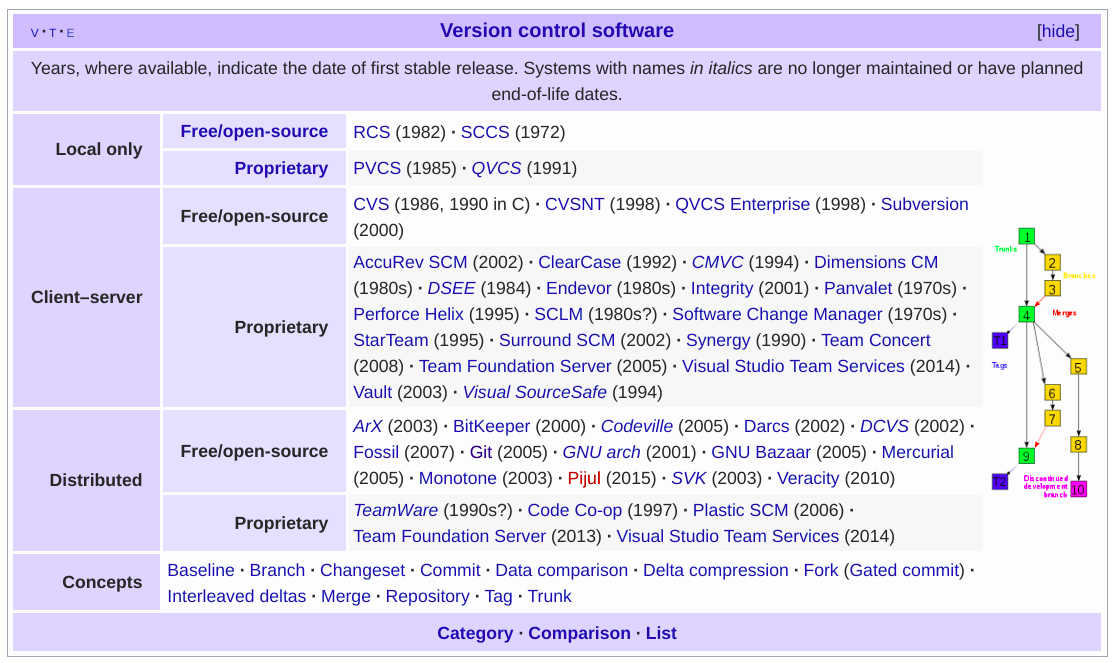
\includegraphics[width=\linewidth]{img/controlVersion.png}
Source: \url{https://en.wikipedia.org/wiki/List_of_version-control_software}
\end{center}
\end{frame}

\begin{frame}[fragile]
    \frametitle{Why use 
\includegraphics[height=12pt]{img/git_logo.png}?}
    \begin{itemize}
        \item { \textbf{Distributed}
            \begin{itemize}
                \item[$-$]{Work online and offline}
                \item[$-$]{Collaborate with large groups}
                \item[$-$]{Fast}
            \end{itemize}
		}         
        \item{ \textbf{Popular and successful}
            \begin{itemize}
                \item[$-$]{Active development}
            \end{itemize}
            }
 
        \item{ \textbf{Tracks any type of files}
            \begin{itemize}
                \item[$-$]{Works best with ASCII files (\verb+.html+, \verb+.tex+, \verb+.R+, \verb+.c+, \verb+.f90+)}
                \item[$-$]{Large binary files with \href{https://git-lfs.github.com/}{Git-LFS} (\verb+.nc+, \verb+.Rdata+, \verb+.mat+, \verb+.csv+)}
            \end{itemize}
            }

        \item { \textbf{Branching}
            \begin{itemize}
                \item[$-$]{Smarter merges}
                \item[$-$]{Easy code management with \href{https://git-flow.readthedocs.io/fr/latest/index.html}{Git-Flow}}
            \end{itemize}
        }
        
       
    \end{itemize}
\end{frame}

\begin{frame}
\frametitle{Git in practice}
\centering
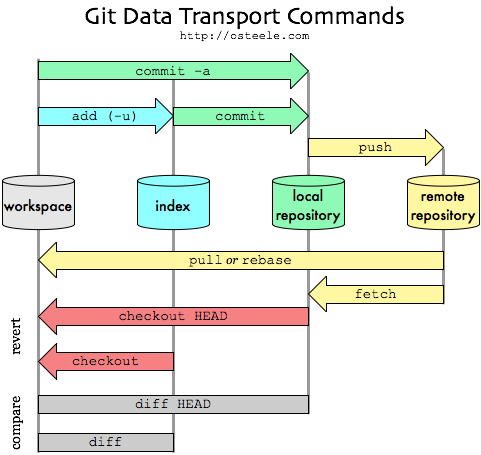
\includegraphics[scale=0.45]{img/MgaV9.png}
\end{frame}

\begin{frame}
\frametitle{Git hosting services}

Several web-based hosting services are available:

\begin{itemize}
\item[$-$]{Commercial: \textbf{\href{https://github.com/}{GitHub}}, \href{https://gitlab.com/}{Gitlab}}
\item[$-$]{Institutional: \href{https://gitlab-bioinfo.ird.fr/}{GitLab Bioinfo}, 
\href{https://gitlab-bioinfo.ird.fr/}{GitLab IRD},
\href{https://gitlab.mbb.univ-montp2.fr/}{GitLab UM},
\href{https://sourcesup.renater.fr/}{SourceSup},
\href{https://forge.ifremer.fr/}{Ifremer Forge}
}



\end{itemize}

Why use 
\includegraphics[height=20pt]{img/GitHub-Mark-120px-plus.png}  ?
\begin{itemize}
\item[$-$] Facilitates worldwide collaboration (no need of institional accounts)
\item[$-$]{Largest host of source code in the world}
\item[$-$]{Free (and improved accounts for education)}
\item[$-$]{Association with Zenodo, Overleaf, LFS, CRAN, PyPI}
%\item[$-$]{Continuous integration (\href{https://github.com/features/actions}{GitHub Actions})}
%\item[$-$]{Institutions (\href{https://github.com/umr-marbec}{Marbec!})}
%\item[$-$]{Hosting personal websites}
%\item[$-$]{Possibility to provide feedbacks (\href{https://docs.github.com/en/github/managing-your-work-on-github/about-issues}{GitHub issues})}
\end{itemize}

\end{frame}

%\begin{frame}[fragile]
%    \frametitle{Git clients}
%
%	\begin{block}{What are Git clients?}
%    IDEs (Integrated Development Environments) to make the experience more pleasant providing a richer visual representation.\\
%    \end{block}
%    \hfill
%
%Some examples:
%\href{https://www.sourcetreeapp.com/}{SourceTreen}, 
%\href{https://www.gitkraken.com/}{GitKraken},
%\href{https://gitup.co/}{GitUp},
%\href{https://www.syntevo.com/smartgit/}{SmartGit}, 
%\href{https://git-cola.github.io/}{git-cola}, 
%\href{https://tortoisegit.org/}{TortoiseGit},
%\href{https://www.rstudio.com/}{RStudio},
%\href{https://code.visualstudio.com/}{VSCode},
%\href{https://netbeans.apache.org/}{NetBeans}\\
%
%\hfill
%
%\begin{alertblock}{Warning!}
%Clients manipulate Git commands (\verb+commit+ , \verb+add+, ...) but in a \emph{hidden} way. 
%Make sure it does the right thing.
%\end{alertblock}
%\hfill
%
%\textbf{In the following, command lines (low level) will be used...}
%
%\end{frame}

\begin{frame}[fragile]
\frametitle{Getting started}

Create a GitHub account on \url{https://github.com}\\
\hfill

Install Git from \url{https://git-scm.com/downloads}\\
\hfill

%{(Install Git LFS from \url{https://git-lfs.github.com/})}\\
%\hfill



Now, open \verb+Git Bash+ (Windows users) or \verb+Terminal+ (Linux/Mac Os X users) and type \verb+which git+. You should see something like this:

\begin{verbatim}
barrier@MPLCLTPO0803 ~ $ which git
/usr/bin/git
\end{verbatim}

\textbf{All set? So let's start!}
\url{https://github.com/umr-marbec/git-training/blob/master/practical-session/Git.md}

\end{frame}

%
%\begin{frame}
%\frametitle{GitHub Inc.}
%  \begin{itemize}
%  \item Work with public and private \textbf{repositories}. 
%  \end{itemize}
%
%\begin{center}
%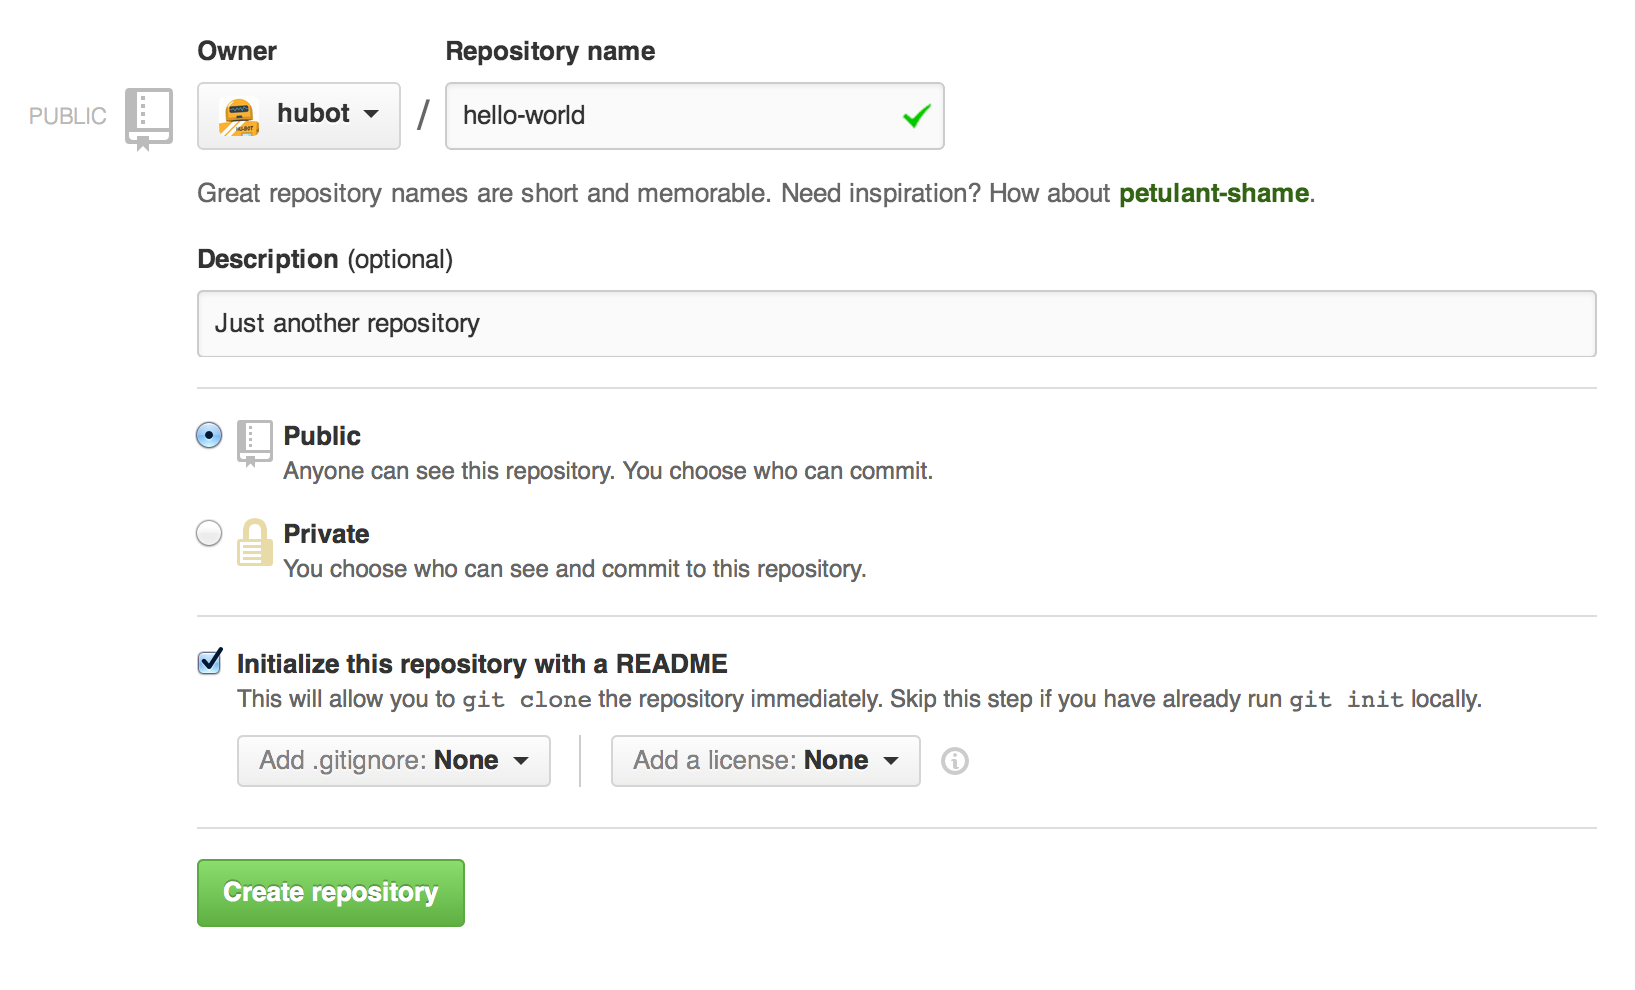
\includegraphics[scale=0.2]{img/githubRepo_features.png}
%\end{center}  
%
%\end{frame}
%
%
%\begin{frame}
%\frametitle{GitHub Inc.}
%\begin{itemize}
%  \item Develop a \textbf{networking}.
%\end{itemize}
%
%\begin{center}
%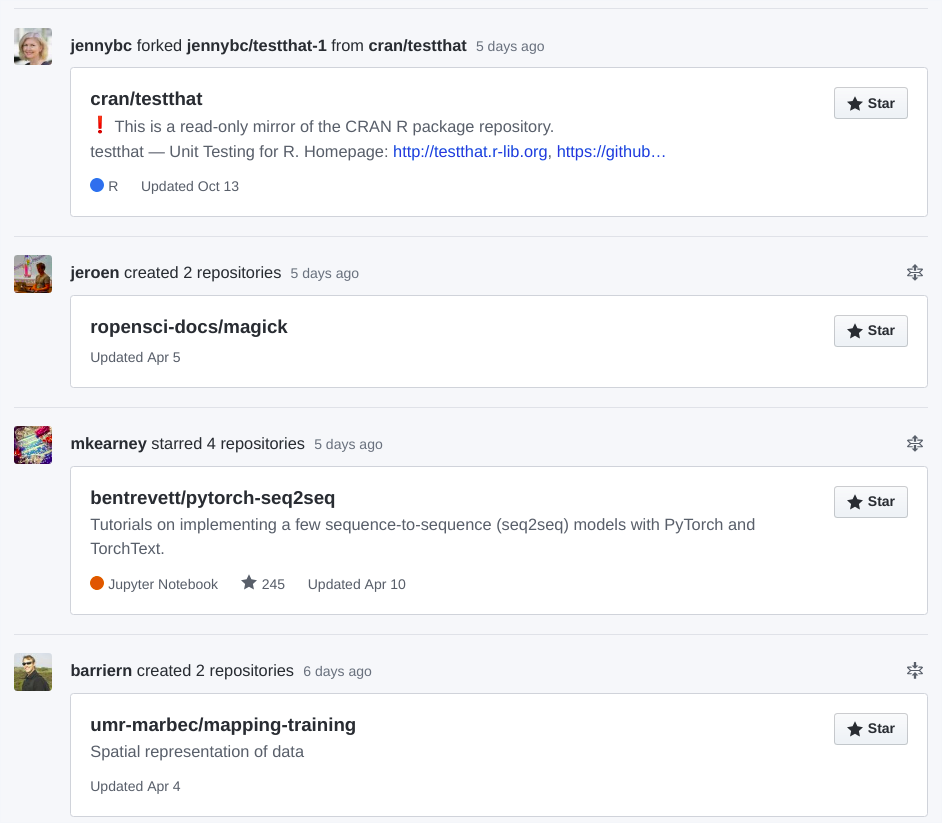
\includegraphics[scale=0.30]{img/githubRepo_networking.png}
%\end{center}  
%
%\end{frame}
%
%\begin{frame}
%\frametitle{GitHub Inc.}
%\begin{itemize}
%  \item Source of information.
%\end{itemize}
%\begin{center}
%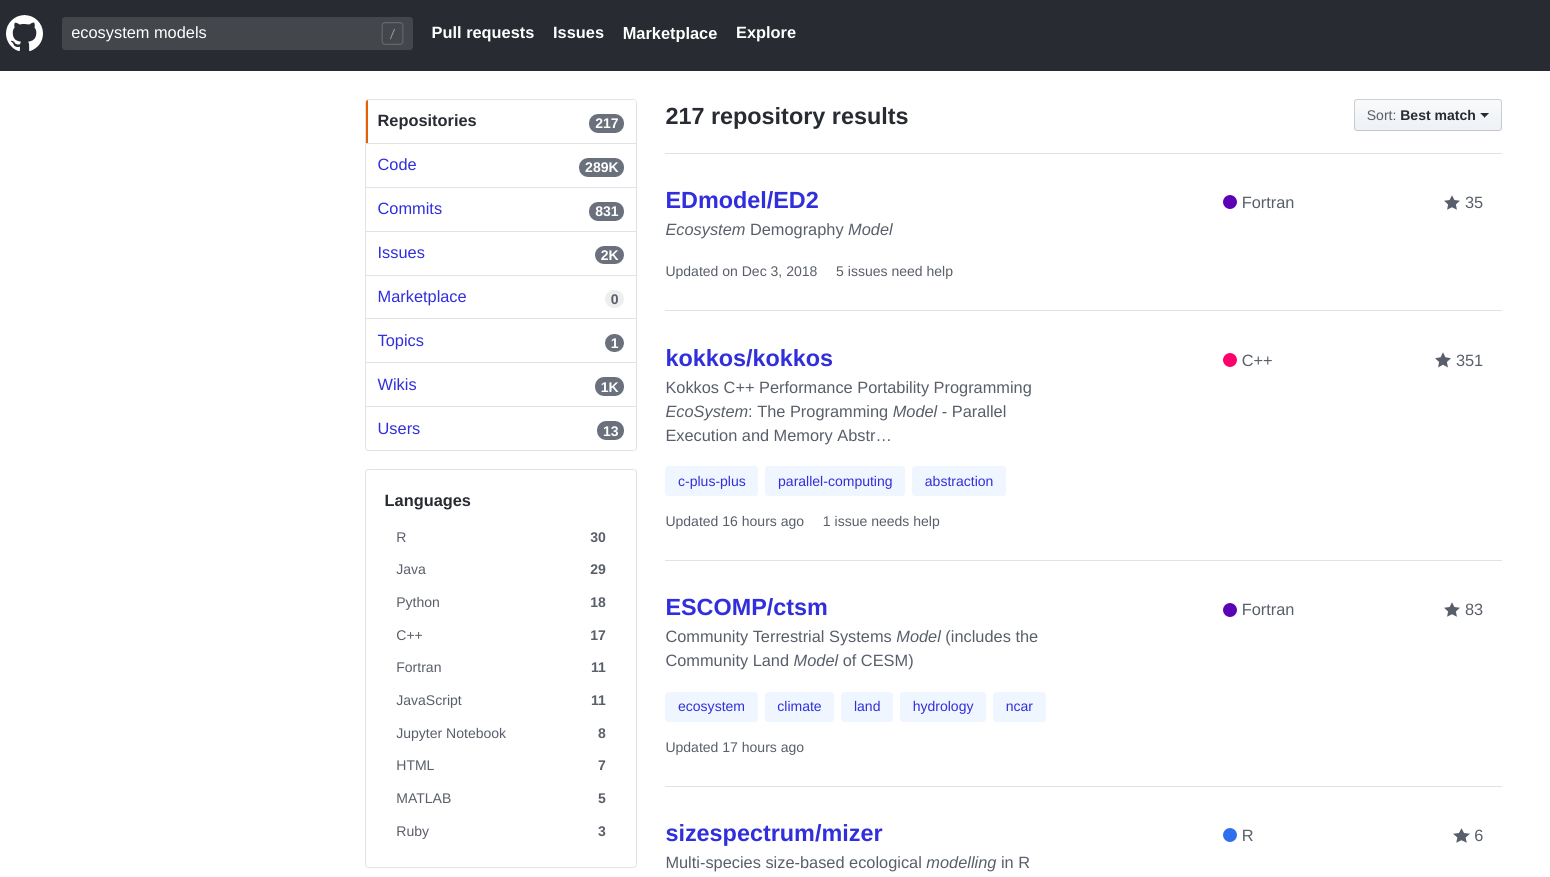
\includegraphics[scale=0.20]{img/github_projects.png}
%\end{center}  
%
%\end{frame}
%
%\begin{frame}
%    \frametitle{GitHub Inc.}
%    \begin{itemize}
%        \item \textbf{Plans} for enterprise, teams, pro and free accounts. \hfill \break
%    \end{itemize}
%
%\begin{center}
%
\includegraphics[scale=0.20]{img/github_plans.png}
%\end{center}  
%
%
%\end{frame}
%
%
%\begin{frame}
%\frametitle{GitHub Inc.}
%\begin{itemize}
%\item Is the \textbf{largest} host of source code in the world! \emph{(28 million users, 57 million repositories (28 million public) - June 2018)}.
%\end{itemize}
%
%\begin{center}
%
\includegraphics[scale=0.35]{img/microsoft-github-800x421.png}
%\end{center}  
%
%\end{frame}
%
%
%\begin{frame}
%\frametitle{Register a GitHub account}
%  \begin{itemize}
%    \item Create an account in \href{https://github.com/}{ GitHub} is free! \hfill \break
%    \item Free private repositories
%        \begin{itemize}
%        \item[$-$] Students, faculty, and educational / research staff: \href{https://education.github.com/}{ GitHub Education}.
%        \item[$-$] Official nonprofit organizations and charities: \href{https://github.com/nonprofit}{ GitHub for Good}.
%       \end{itemize}
%        
%\end{itemize}
%\end{frame}
%
%\begin{frame}
%\frametitle{Register a GitHub account}
%\begin{itemize}
%    \item Pay for private repositories
%    \begin{itemize}
%    \item[$-$] Individual cost is 7 dollars per month: \href{https://github.com/pricing}{ GitHub Pricing}.
%    \end{itemize}
%
%\end{itemize}
%
%\begin{center}
%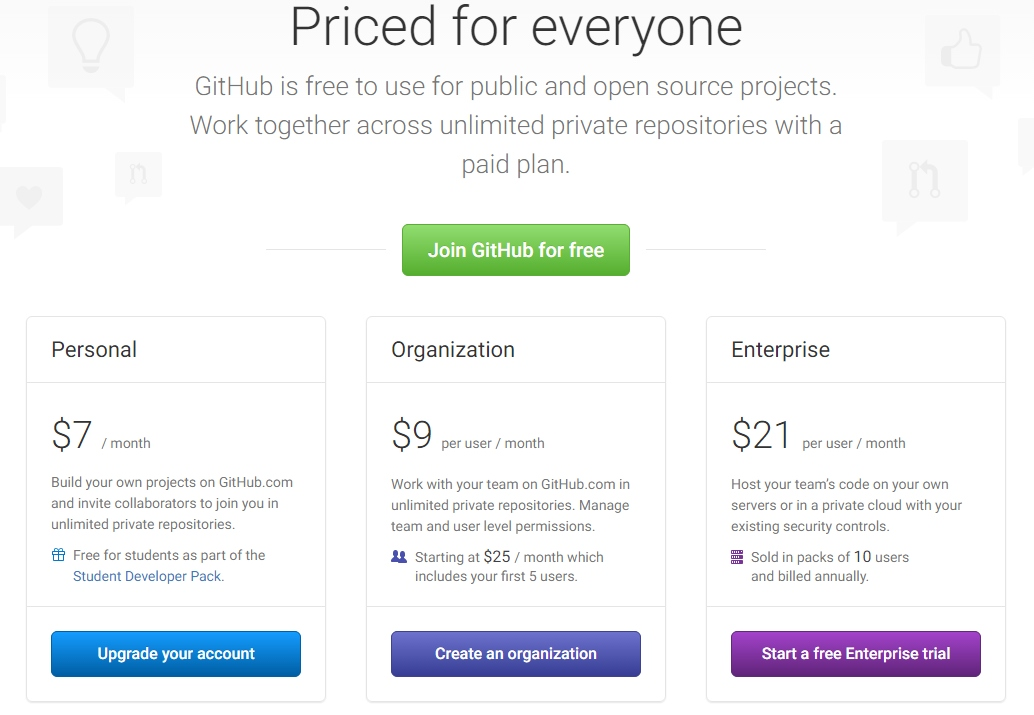
\includegraphics[scale=0.35]{img/github_pricing.jpg}
%\end{center}  
%\end{frame}
%
%\begin{frame}
%\frametitle{Marbec in GitHub}
%
%    All the materials of Pole Modelisation's technical "workshop" are now stored in an institutionnal GitHub account: \url{https://github.com/umr-marbec}.
%
%\begin{center}
%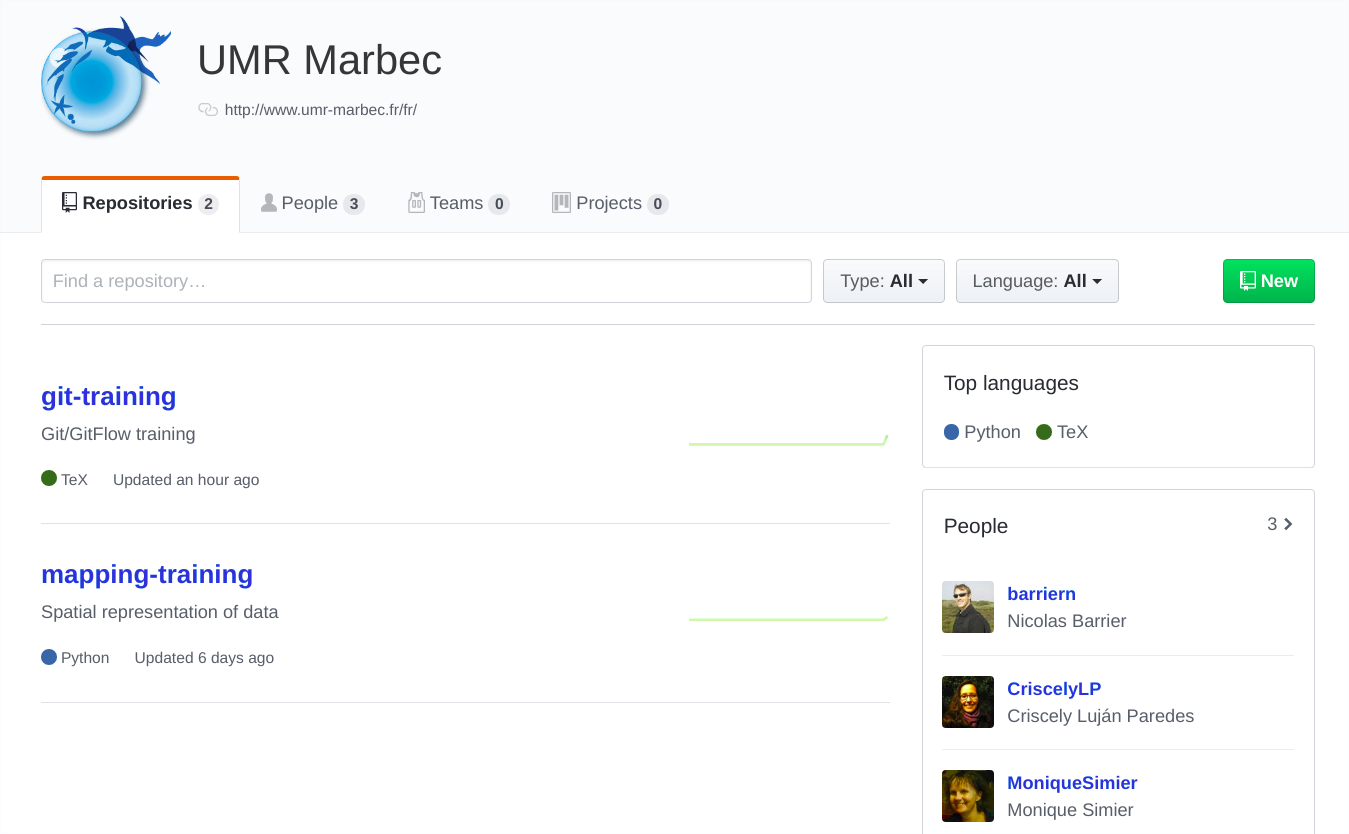
\includegraphics[scale=0.2]{img/github_marbec.png}
%\end{center}  
%\end{frame}
%
%\begin{frame}
%    \frametitle{Institutionnal repositories}
%
%    GitHub is a private US company. There are also \emph{institutional} repositories on which Git can be used:
%
%    \begin{itemize}
%        \item{\href{https://sourcesup.renater.fr/}{Sourcesup}: this is a Renater platform (login possible from any French research institute or through CRU accounts)}
%        \item{\href{https://forge.ifremer.fr/}{Forge Ifremer}: very close to SourceSup (Ifremer extranet account required)}
%        \item{\href{gitlab.intranet.ird.fr}{IRD GitLab}: GitLab IRD platform (IRD account required).}
%    \end{itemize}
%
%    However, the projects hosted on these repositories may have less visibility...
%
%\end{frame}
%
%
%\begin{frame}
%    \frametitle{Git clients}
%
%    Git and Git client \textbf{are not} the same! Like R and RStudio is not the same thing!
%    \hfill \break
%
%    Git client:
%    \begin{itemize}
%        \item IDE (Integrated development environment)!
%        \item Make the experience more pleasant providing a richer visual representation.
%    \end{itemize}
%
%    \hfill 
%
%    Some example of Git clients:
%    \begin{itemize}
%        \item \href{https://www.sourcetreeapp.com/}{ SourceTreen} 
%        \item \href{https://www.gitkraken.com/}{ GitKraken}
%        \item \href{https://gitup.co/}{ GitUp} 
%        \item \href{https://www.syntevo.com/smartgit/}{ SmartGit} 
%        \item \href{https://git-cola.github.io/}{ git-cola} 
%        \item \href{https://www.rstudio.com/}{ RStudio}
%    \end{itemize}
%
%    \vspace{3em}
%
%\end{frame}
%
%\begin{frame}[fragile]
%    \frametitle{Git branches}
%    One main advantage of Git is the use of \emph{branches}, which allow multiple developments of the same code at the same time.
%
%    \begin{block}{Definition}
%        A branch in Git is simply a lightweight movable pointer to one of thes commits.
%    \end{block}
%    
%    \begin{center}
%        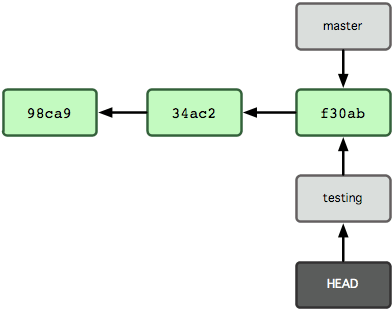
\includegraphics[height=2.5cm]{img/git-branch-ter.png}
%        \hspace{3em}
%        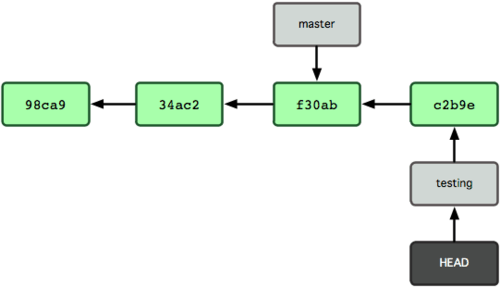
\includegraphics[height=2.5cm]{img/git-branch-bis.png}
%    \end{center}
%
%    In this example, the \verb+master+ branch points to the \verb+f30ab+ commit, while the \verb+testing+ branch points to the \verb+c2b9e+ one. \verb+HEAD+ points
%    to the active branch (here, \verb+testing+).
%
%    \vspace{1em}
%    \tiny Source: \url{https://git-scm.com/book/en/v1/Git-Branching-What-a-Branch-Is}
%
%\end{frame}
%
%\begin{frame}[fragile]
%    \frametitle{Merging branches}
%    To merge a branch (for instance a feature branch) to another branch (for instance the main one), several options are offered.
%    \begin{itemize}
%        \item{\verb+merge+: Three-points branch (common ancestor + tips of the two branches)} 
%        \item{\verb+rebase+: Compresses all the changes into a single “patch.” }
%    \end{itemize}
%
%    \begin{center}
%        \begin{figure}
%            \subfloat[Merge]{
%                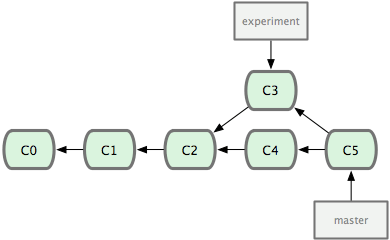
\includegraphics[scale=0.3]{img/git-merge-1.png}
%                \label{git-merge}
%            }
%            \hspace{3em}
%            \subfloat[Rebase]{
%                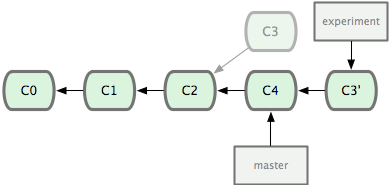
\includegraphics[scale=0.3]{img/git-merge-2.png}
%                \label{git-rebase}
%            }
%            \caption{Merging versus rebasing}
%        \end{figure}
%    \end{center}
%
%    \tiny Source: \url{https://git-scm.com/book/fr/v1/Les-branches-avec-Git-Rebaser}
%
%\end{frame}
%
%\begin{frame}
%    \frametitle{Git workflows} % Table of contents slide, comment this block out to remove it
%    There are several ways to use Git branches (we talk about \textbf{workflows}). 
%
%    \begin{itemize}
%        \item \emph{Centralized workflow}: one main branch, everyone commit in the same place.
%        \item \emph{Feature Branch Workflow}: developments are made in dedicated branches (feature branches), which are regularly merged into the master one.
%        \item \textbf{\textit{Gitflow Workflow}}: Strict branching model designed around the project release.
%    \end{itemize}
%
%    \tiny Source: \url{https://www.atlassian.com/git/tutorials/comparing-workflows}
%
%\end{frame}
%
%\begin{frame}[fragile]{GitFlow branches}
%
%    GitFlow workflow contains two main branches:
%    \begin{itemize}
%        \item{\verb+master+: official release history. Branch which is shared to the world!}
%        \item{\verb+develop+: integration branch for features}
%    \end{itemize}
%
%    It also contains additional temporal branches:
%    \begin{itemize}
%        \item{\verb+feature+: feature branches (one for each new feature to add to the code)}
%        \item{\verb+release+: branch created when enough features have been added (new version of the code) to develop}
%        \item{\verb+hotfix+: branch for maintenance and bug correction of the production release}
%    \end{itemize}
%
%\end{frame}
%
%\begin{frame}{In summary...}
%
%    \begin{center}
%        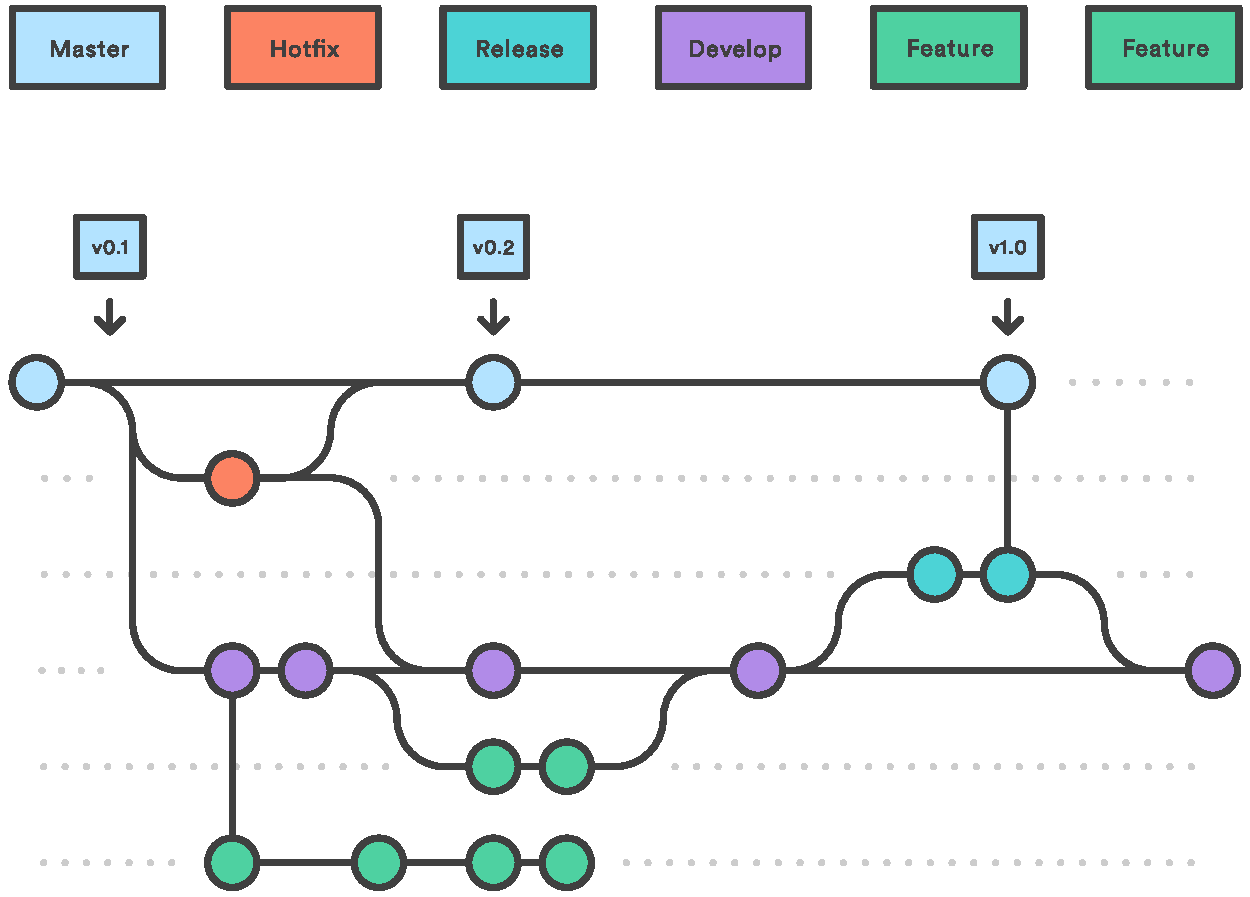
\includegraphics[scale=0.5]{img/05-_2_.pdf}    
%    \end{center}
%    
%    \tiny Source: \url{https://www.atlassian.com/git/tutorials/comparing-workflows}
%
%\end{frame}    
%
%
%\begin{frame}
%    \frametitle{Thanks for your attention} % Table of contents slide, comment this block out to remove it
%
%            \begin{center}
%                \textbf{Now, let's crack on it!}\\
%                \vspace{2em}
%
%                
\includegraphics[scale=0.55]{img/funny.jpg}\\
%                \vspace{1em}
%                \tiny Source: \url{https://www.pinterest.fr/pin/447263806724736402/}
%            \end{center}
%\end{frame}
%
%\begin{frame}
%    \frametitle{This is the end} % Table of contents slide, comment this block out to remove it
%
%            \begin{center}
%                
%                
\includegraphics[scale=0.15]{img/that_s_all_folks.png}\\
%                \vspace{1em}
%                \tiny Source: \url{poshpete117.deviantart.com/journal/Thats-All-Folks-427323458/}
%            \end{center}
%\end{frame}



\end{document}
